\documentclass[12pt]{article}
\usepackage{amsmath}
\usepackage{latexsym}
\usepackage{amsfonts}
\usepackage[normalem]{ulem}
\usepackage{array}
\usepackage{amssymb}
\usepackage{graphicx}
\usepackage[backend=biber,
style=numeric,
sorting=none,
isbn=false,
doi=false,
url=false,
]{biblatex}\addbibresource{bibliography.bib}


\usepackage{subfig}
\usepackage{wrapfig}
\usepackage{wasysym}
\usepackage{enumitem}
\usepackage{adjustbox}
\usepackage{ragged2e}
\usepackage[svgnames,table]{xcolor}
\usepackage{tikz}
\usepackage{longtable}
\usepackage{changepage}
\usepackage{setspace}
\usepackage{hhline}
\usepackage{multicol}
\usepackage{tabto}
\usepackage{float}
\usepackage{multirow}
\usepackage{makecell}
\usepackage{fancyhdr}
\usepackage[toc,page]{appendix}
\usepackage[hidelinks]{hyperref}
\usetikzlibrary{shapes.symbols,shapes.geometric,shadows,arrows.meta}
\tikzset{>={Latex[width=1.5mm,length=2mm]}}
\usepackage{flowchart}\usepackage[paperheight=11.69in,paperwidth=8.27in,left=1.18in,right=1.18in,top=0.98in,bottom=0.98in,headheight=1in]{geometry}
\usepackage[utf8]{inputenc}
\usepackage[T1]{fontenc}
\TabPositions{0.49in,0.98in,1.47in,1.96in,2.45in,2.94in,3.43in,3.92in,4.41in,4.9in,5.39in,5.88in,}
\urlstyle{same}


 %%%%%%%%%%%%  Set Depths for Sections  %%%%%%%%%%%%%%

% 1) Section
% 1.1) SubSection
% 1.1.1) SubSubSection
% 1.1.1.1) Paragraph
% 1.1.1.1.1) Subparagraph


\setcounter{tocdepth}{5}
\setcounter{secnumdepth}{5}


 %%%%%%%%%%%%  Set Depths for Nested Lists created by \begin{enumerate}  %%%%%%%%%%%%%%


\setlistdepth{9}
\renewlist{enumerate}{enumerate}{9}
		\setlist[enumerate,1]{label=\arabic*)}
		\setlist[enumerate,2]{label=\alph*)}
		\setlist[enumerate,3]{label=(\roman*)}
		\setlist[enumerate,4]{label=(\arabic*)}
		\setlist[enumerate,5]{label=(\Alph*)}
		\setlist[enumerate,6]{label=(\Roman*)}
		\setlist[enumerate,7]{label=\arabic*}
		\setlist[enumerate,8]{label=\alph*}
		\setlist[enumerate,9]{label=\roman*}

\renewlist{itemize}{itemize}{9}
		\setlist[itemize]{label=$\cdot$}
		\setlist[itemize,1]{label=\textbullet}
		\setlist[itemize,2]{label=$\circ$}
		\setlist[itemize,3]{label=$\ast$}
		\setlist[itemize,4]{label=$\dagger$}
		\setlist[itemize,5]{label=$\triangleright$}
		\setlist[itemize,6]{label=$\bigstar$}
		\setlist[itemize,7]{label=$\blacklozenge$}
		\setlist[itemize,8]{label=$\prime$}

\setlength{\topsep}{0pt}\setlength{\parskip}{8.04pt}
\setlength{\parindent}{0pt}

 %%%%%%%%%%%%  This sets linespacing (verticle gap between Lines) Default=1 %%%%%%%%%%%%%%


\renewcommand{\arraystretch}{1.3}


%%%%%%%%%%%%%%%%%%%% Document code starts here %%%%%%%%%%%%%%%%%%%%



\begin{document}

% \author{}
\title{Caratula}

\begin{titlepage}
\begin{center}
\large{UNIVERSIDAD PRIVADA DE TACNA}\\
\vspace*{0.1in}
\begin{figure}[htb]
\begin{center}

\includegraphics[width=6cm]{./media/logo_upt}
\end{center}
\end{figure}
\vspace*{0.15in}
INGENIERIA DE SISTEMAS  \\



\vspace*{0.5in}
\begin{large}
TITULO:\\
\end{large}

\vspace*{0.1in}
\begin{Large}
\textbf{TRABAJO FINAL UNIDAD I - BIBLIOTECA} \\
\end{Large}

\vspace*{0.3in}
\begin{Large}
\textbf{CURSO:} \\
\end{Large}

\vspace*{0.1in}
\begin{large}
BASE DE DATOS II\\
\end{large}

\vspace*{0.3in}
\begin{Large}
\textbf{DOCENTE(ING):} \\
\end{Large}

\vspace*{0.1in}
\begin{large}
 Patrick Cuadros Quiroga\\
\end{large}

\vspace*{0.2in}
\vspace*{0.1in}
\begin{large}
Integrantes: \\
\begin{flushleft}

Condori Gutierrez,Flor de Maria            	\hfill	(2015053227) \\

\end{flushleft}
\end{large}
\end{center}

\end{titlepage}

\begin{center}
\begin{Large}
\textbf{TRABAJO FINAL\\
\vspace*{0.42in}
SISTEMA BIBLIOTECA} 
\end{Large}
\end{center}
\vspace{\baselineskip}
\begin{enumerate}[label*=\arabic*.]

\vspace{\baselineskip}

    \item PROBLEMA \par
    
\vspace{\baselineskip}
	

\vspace{\baselineskip}
{\fontsize{13pt}{15.6pt}\selectfont Nos pide sistematizar una biblioteca, para una determinada reservación, o prestamos de algún libro y atención a los usuarios de la universidad de manera satisfactoria y darle una solución a través del visual studio.\  \par}\par

{\fontsize{13pt}{15.6pt}\selectfont 1.1. Titulo Descriptivo del Proyecto\par}\par

\begin{adjustwidth}{0.35in}{0.0in}{\fontsize{13pt}{15.6pt}\selectfont Para este proyecto, tiene como nombre BIBLIOTECA que esto forma parte de la sistematización de la biblioteca de la upt. podría ser en alguna otra biblioteca que lo necesiten este tipo de modelo, que será desarrollado de manera grupal y sería más que todo en nuestras casas o en la universidad misma donde lo desarrollaremos.\par}\par

\end{adjustwidth}

{\fontsize{13pt}{15.6pt}\selectfont 1.2. Formulación del Problema\par}\par

\begin{adjustwidth}{0.35in}{0.0in}

{\fontsize{13pt}{15.6pt}\selectfont Para la solución del problema de este dicho proyecto sería más que todo para que los usuarios se sientan conforme con la atención que le damos con este software y así no tenga ninguna queja al momento de ingresar a la biblioteca virtual.\par}\par

\end{adjustwidth}

\vspace{\baselineskip}

    \item MARCO TEÓRICO \par
    
\vspace{\baselineskip}

{\fontsize{13pt}{15.6pt}\selectfont 2.1. MVC\par}\par

\begin{adjustwidth}{0.35in}{0.0in}
{\fontsize{13pt}{15.6pt}\selectfont En este diseño de biblioteca de software utilizada para implementar sistemas donde se requiere el uso de interfaces de usuario. Surge de la necesidad de crear software más robusto con un ciclo de vida más adecuado, donde se potencie la facilidad de mantenimiento, reutilización del código y la separación de conceptos.\par}\par

{\fontsize{13pt}{15.6pt}\selectfont Su fundamento es la separación del código en tres capas diferentes, acotadas por su responsabilidad, en lo que se llaman Modelos, Vistas y Controladores, o lo que es lo mismo, Model, Views $\&$  Controllers, si lo prefieres en inglés. \par}\par

{\fontsize{13pt}{15.6pt}\selectfont MVC es un "invento" que ya tiene varias décadas y fue presentado incluso antes de la aparición de la Web. No obstante, en los últimos años ha ganado mucha fuerza y seguidores gracias a la aparición de numerosos frameworks de desarrollo web que utilizan el patrón MVC como modelo para la arquitectura de las aplicaciones web.\par}\par

\end{adjustwidth}

{\fontsize{13pt}{15.6pt}\selectfont 2.2. Entity Framework \par}\par

\begin{adjustwidth}{0.35in}{0.0in}
{\fontsize{13pt}{15.6pt}\selectfont Es un conjunto de tecnologías de ADO.NET que permiten el desarrollo de aplicaciones de software orientadas a datos. Los arquitectos y programadores de aplicaciones orientadas a datos se han enfrentado a la necesidad de lograr dos objetivos muy diferentes. Deben modelar las entidades, las relaciones y la lógica de los problemas empresariales que resuelven, y también deben trabajar con los motores de datos que se usan para almacenar y recuperar los datos. Los datos pueden abarcar varios sistemas de almacenamiento, cada uno con sus propios protocolos; incluso las aplicaciones que funcionan con un único sistema de almacenamiento deben equilibrar los requisitos del sistema de almacenamiento con respecto a los requisitos de escribir un código de aplicación eficaz y fácil de mantener.\par}\par

{\fontsize{13pt}{15.6pt}\selectfont Entity Framework permite a los desarrolladores trabajar con datos en forma de objetos y propiedades específicos del dominio, como clientes y direcciones de cliente, sin tener que preocuparse por las tablas y columnas de la base de datos subyacente donde se almacenan estos datos. Con Entity Framework, los desarrolladores pueden trabajar en un nivel mayor de abstracción cuando tratan con datos, y pueden crear y mantener aplicaciones orientadas a datos con menos código que en las aplicaciones tradicionales. Dado que Entity Framework es un componente de .NET Framework, las aplicaciones de Entity Framework se pueden ejecutar en cualquier equipo en el que esté instalado .NET Framework a partir de la versión 3.5 SP1.\par}\par

\end{adjustwidth}


\vspace{\baselineskip}
	\item DESARROLLO\par

\begin{enumerate}[label*=\arabic*.]
	\item Análisis\par
	\vspace{\baselineskip}
\begin{itemize}
	

\item Requerimientos funcionales \par



%%%%%%%%%%%%%%%%%%%% Table No: 1 starts here %%%%%%%%%%%%%%%%%%%%


\begin{table}[H]
 			\centering
\begin{tabular}{p{1.2in}p{0.4in}p{1.0in}p{1.99in}p{0.51in}}
\hline
%row no:1
\multicolumn{1}{|p{1.2in}}{Módulos} & 
\multicolumn{1}{|p{0.50in}}{Código} & 
\multicolumn{1}{|p{1.16in}}{Requerimientos} & 
\multicolumn{1}{|p{1.99in}}{Descripción} & 
\multicolumn{1}{|p{0.65in}|}{Prioridad} \\
\hhline{-----}
%row no:2
\multicolumn{1}{|p{1.2in}}{\multirow{1}{*}{\begin{tabular}{p{1.2in}} \textbf{MANTENI-MIENTO}\\\end{tabular}}} & 
\multicolumn{1}{|p{0.4in}}{RF-01} & 
\multicolumn{1}{|p{1.0in}}{Buscar Libro} & 
\multicolumn{1}{|p{1.99in}}{El sistema le permitirá al usuario realizar la búsqueda del libro, ya sea por el nombre del libro o alguna característica que el sistema tendrá en su interfaz. } & 
\multicolumn{1}{|p{0.51in}|}{ALTA \par } \\
\hhline{~----}
%row no:3
\multicolumn{1}{|p{1.2in}}{} & 
\multicolumn{1}{|p{0.4in}}{RF-02} & 
\multicolumn{1}{|p{1.0in}}{Reservar Libro} & 
\multicolumn{1}{|p{1.99in}}{El sistema le permitirá al usuario realizar la reserva de un libro.} & 
\multicolumn{1}{|p{0.51in}|}{ALTA} \\
\hhline{-----}
%row no:4
\multicolumn{1}{|p{1.2in}}{} & 
\multicolumn{1}{|p{0.4in}}{RF-03} & 
\multicolumn{1}{|p{1.0in}}{Cancelar Libro} & 
\multicolumn{1}{|p{1.99in}}{El sistema le permitirá al usuario cancelar el libro que ya reservo. } & 
\multicolumn{1}{|p{0.51in}|}{ALTA} \\
\hhline{-----}
%row no:5
\multicolumn{1}{|p{1.2in}}{} & 
\multicolumn{1}{|p{0.4in}}{RF-04} & 
\multicolumn{1}{|p{1.0in}}{Agregar Favorito} & 
\multicolumn{1}{|p{1.99in}}{El sistema le permitirá al usuario poner en su lista los libros favoritos, según criterio de cada usuario.} & 
\multicolumn{1}{|p{0.51in}|}{ALTA} \\
\hhline{-----}
%row no:6
\multicolumn{1}{|p{1.2in}}{} & 
\multicolumn{1}{|p{0.4in}}{RF-05} & 
\multicolumn{1}{|p{1.0in}}{Eliminar Favoritos} & 
\multicolumn{1}{|p{1.99in}}{El sistema le permitirá al usuario eliminar de los favoritos los libros que no sean de su agrado.} & 
\multicolumn{1}{|p{0.51in}|}{ALTA} \\
\hhline{-----}
%row no:7
\multicolumn{1}{|p{1.2in}}{} & 
\multicolumn{1}{|p{0.4in}}{RF-06} & 
\multicolumn{1}{|p{1.0in}}{Gestionar Libro} & 
\multicolumn{1}{|p{1.99in}}{El sistema le permitirá al administrador realizar la parte de gestionar (actualizar, guardar, eliminar, etc).} & 
\multicolumn{1}{|p{0.51in}|}{ALTA} \\
\hhline{-----}
%row no:8
\multicolumn{1}{|p{1.2in}}{} & 
\multicolumn{1}{|p{0.4in}}{RF-07} & 
\multicolumn{1}{|p{1.0in}}{Registrar entrega libro} & 
\multicolumn{1}{|p{1.99in}}{El sistema le permitirá al empleado registrar el préstamo del libro, el cual se le entregara al usuario.} & 
\multicolumn{1}{|p{0.51in}|}{ALTA} \\
\hhline{-----}
%row no:9
\multicolumn{1}{|p{1.2in}}{} & 
\multicolumn{1}{|p{0.4in}}{RF-08} & 
\multicolumn{1}{|p{1.0in}}{Registrar\ devolución libro  } & 
\multicolumn{1}{|p{1.99in}}{El sistema le permitirá al empleado registrar la devolución del libro del usuario.} & 
\multicolumn{1}{|p{0.51in}|}{ALTA} \\
\hhline{-----}
%row no:10
\multicolumn{1}{|p{1.2in}}{\Centering \textbf{SEGURIDAD}} & 
\multicolumn{1}{|p{0.4in}}{RF-24} & 
\multicolumn{1}{|p{1.0in}}{Autenticación} & 
\multicolumn{1}{|p{1.99in}}{El usuario, administrador y empleado ingresar al sistema mediante la identificación de.} & 
\multicolumn{1}{|p{0.51in}|}{ALTA} \\
\hhline{-----}

\end{tabular}
 \end{table}


%%%%%%%%%%%%%%%%%%%% Table No: 1 ends here %%%%%%%%%%%%%%%%%%%%

\newpage

	\item Caso de uso \par

Este diagrama demuestra todos los requerimientos o casos de usos que existen en el proyecto de Bilioteca.

%%%%%%%%%%%%%%%%%%%% Figure/Image No: 1 starts here %%%%%%%%%%%%%%%%%%%%
\begin{figure}[H]
	\begin{Center}
		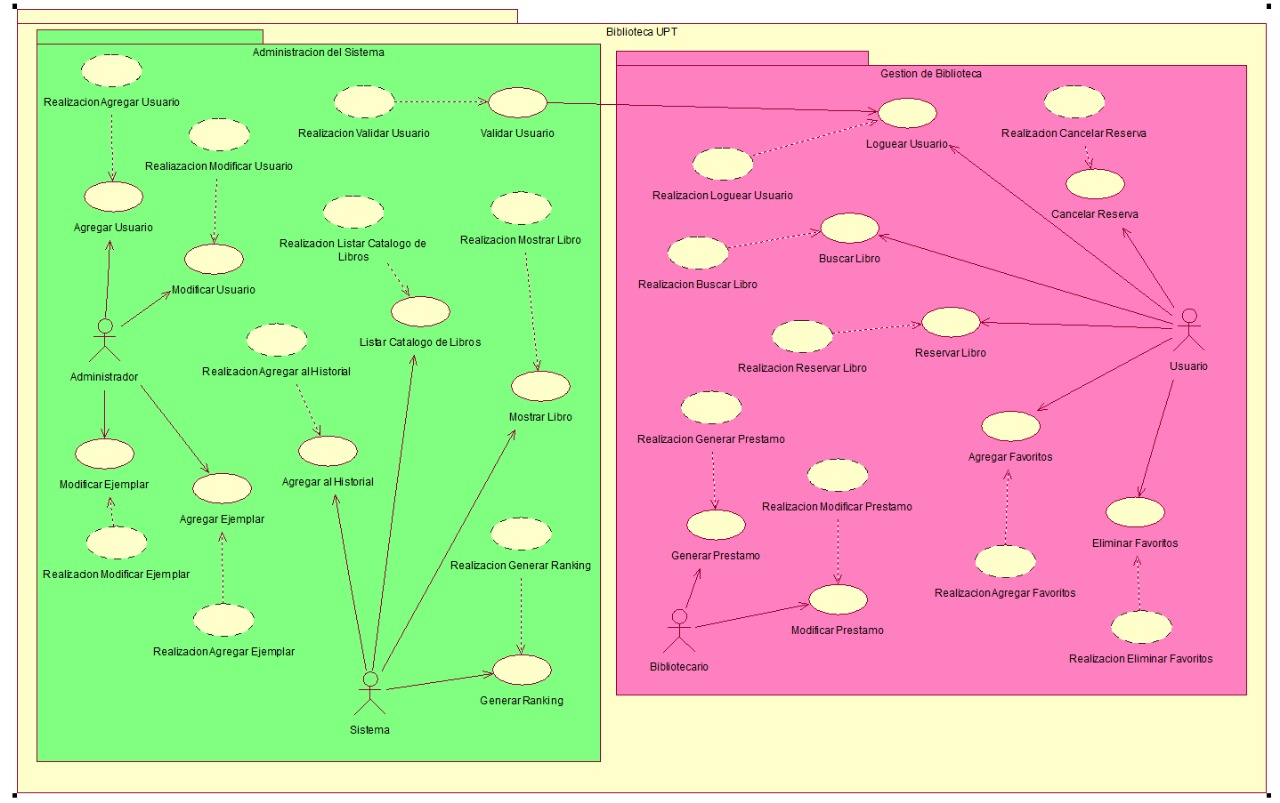
\includegraphics[width=6in,height=4in]{./media/cDeUso.jpg}
	\end{Center}
\end{figure}

%%%%%%%%%%%%%%%%%%%% Figure/Image No: 1 Ends here %%%%%%%%%%%%%%%%%%%%



\newpage

\par

	\item Modelo entidad relación  

Este diagrama es muestra la cardinalidad, relaciones y atributos de las Clases  existentes en el proyecto. Este diagrama fue hecho en Erwin Data Modeler.
\vspace{\baselineskip}


%%%%%%%%%%%%%%%%%%%% Figure/Image No: 4 starts here %%%%%%%%%%%%%%%%%%%%

\begin{figure}[H]
	\begin{Center}
		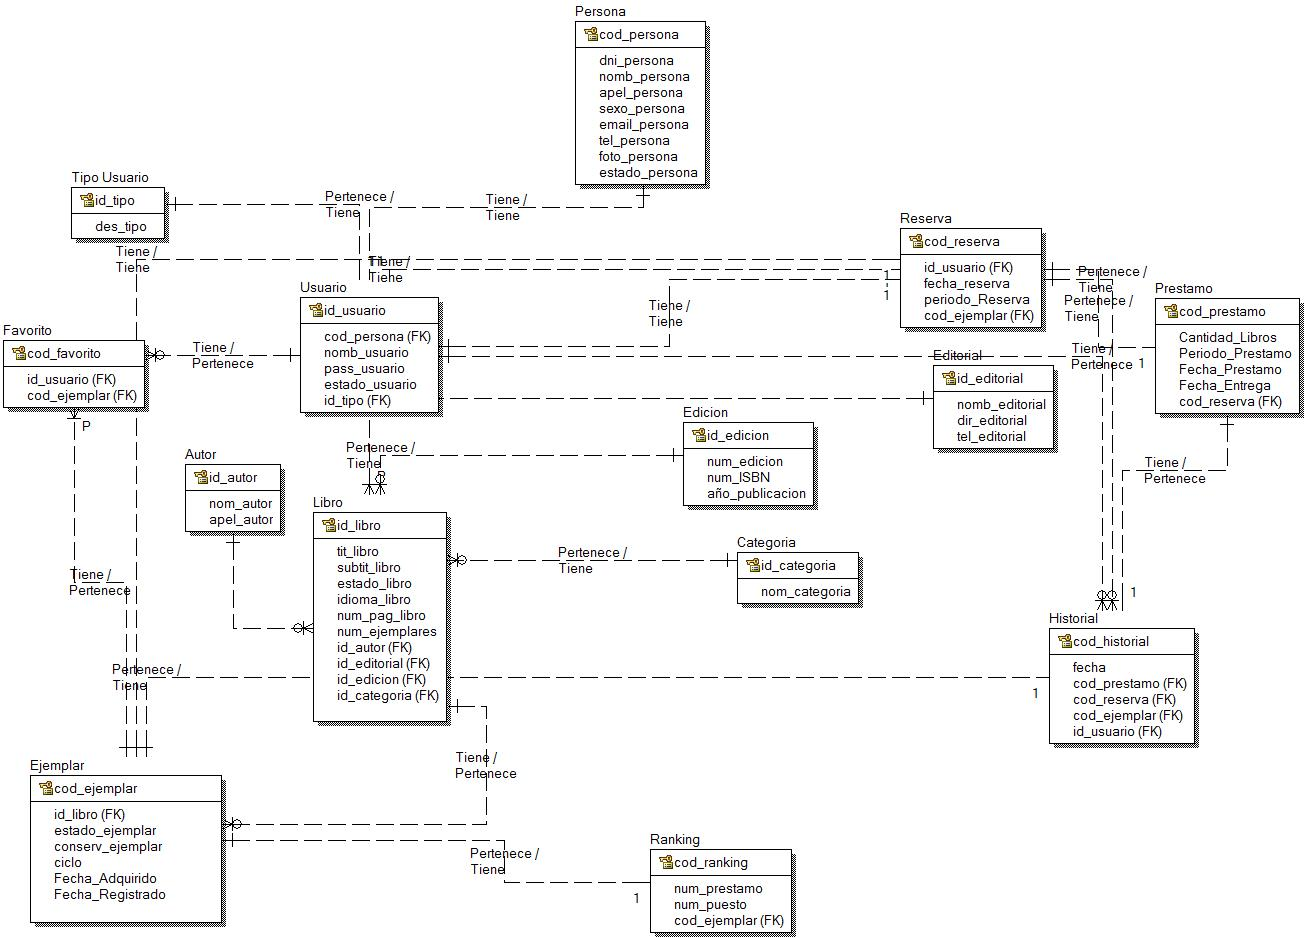
\includegraphics[width=5.91in,height=4.25in]{./media/figura4.jpg}
	\end{Center}
\end{figure}


%%%%%%%%%%%%%%%%%%%% Figure/Image No: 4 Ends here %%%%%%%%%%%%%%%%%%%%

\par
\end{itemize}

	\item ENTIDADES
\vspace{\baselineskip}

Clase Autor:
\begin{figure}[H]
	\begin{Center}
		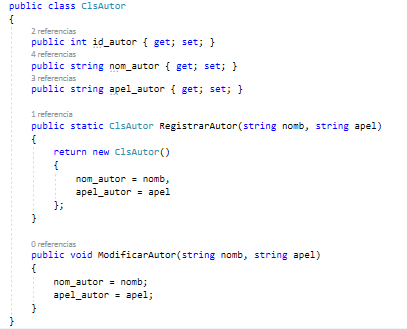
\includegraphics[width=4.91in,height=3.15in]{./media/1.png}
	\end{Center}
\end{figure}

\newpage
Clase Categoria:
\begin{figure}[H]
	\begin{Center}
		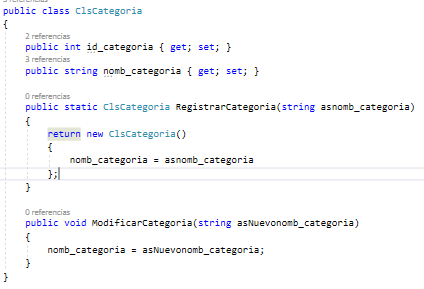
\includegraphics[width=4.91in,height=3.15in]{./media/2.png}
	\end{Center}
\end{figure}


Clase Edicion:
\begin{figure}[H]
	\begin{Center}
		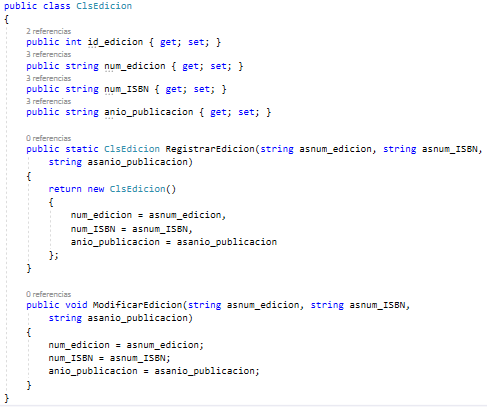
\includegraphics[width=4.91in,height=4.15in]{./media/3.png}
	\end{Center}
\end{figure}

\newpage
Clase Editorial:
\begin{figure}[H]
	\begin{Center}
		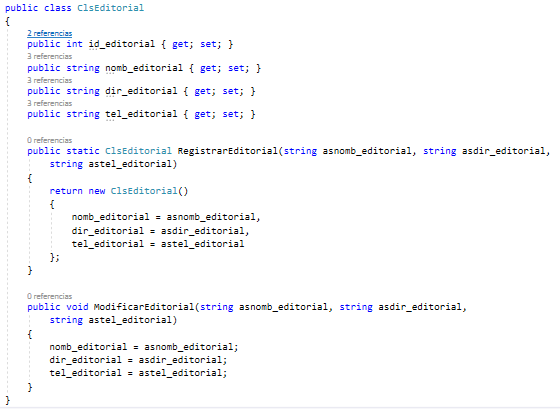
\includegraphics[width=4.91in,height=4.15in]{./media/4.png}
	\end{Center}
\end{figure}


Clase Ejemplar:
\begin{figure}[H]
	\begin{Center}
		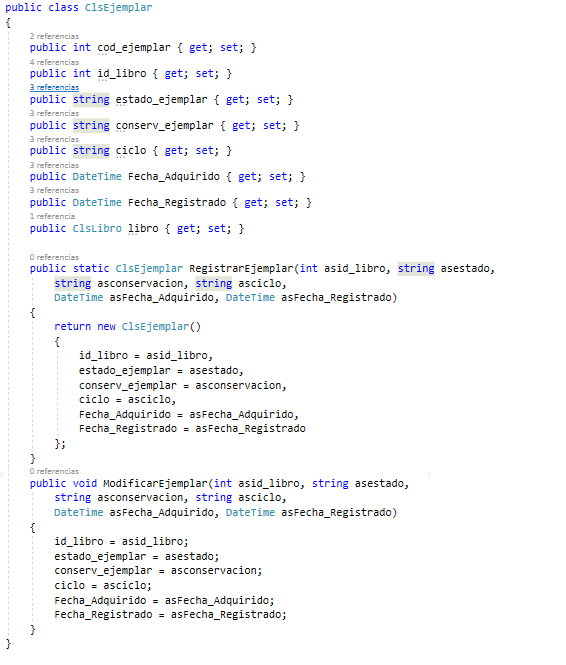
\includegraphics[width=4.91in,height=4.35in]{./media/5.png}
	\end{Center}
\end{figure}


\newpage
Clase Favorito:
\begin{figure}[H]
	\begin{Center}
		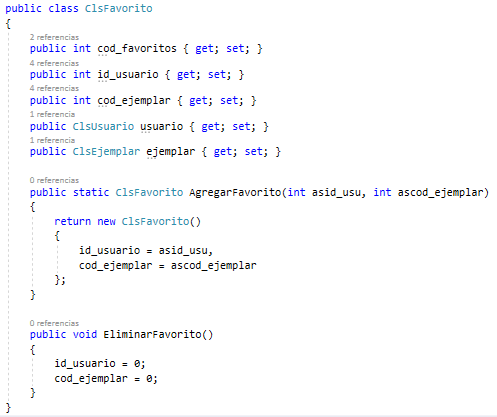
\includegraphics[width=4.91in,height=4.15in]{./media/6.png}
	\end{Center}
\end{figure}


Clase Historial:
\begin{figure}[H]
	\begin{Center}
		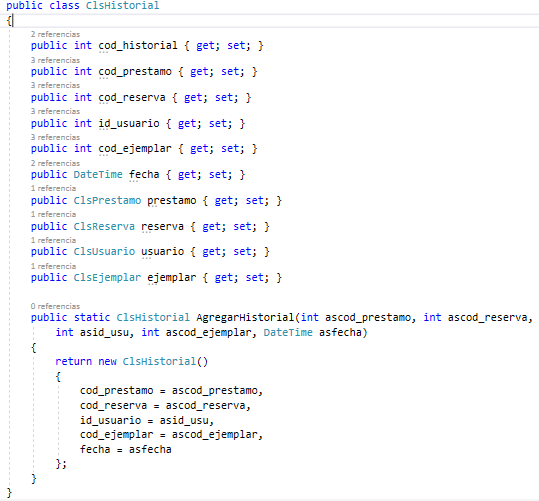
\includegraphics[width=4.91in,height=4.35in]{./media/7.png}
	\end{Center}
\end{figure}

\newpage
Clase Libror:
\begin{figure}[H]
	\begin{Center}
		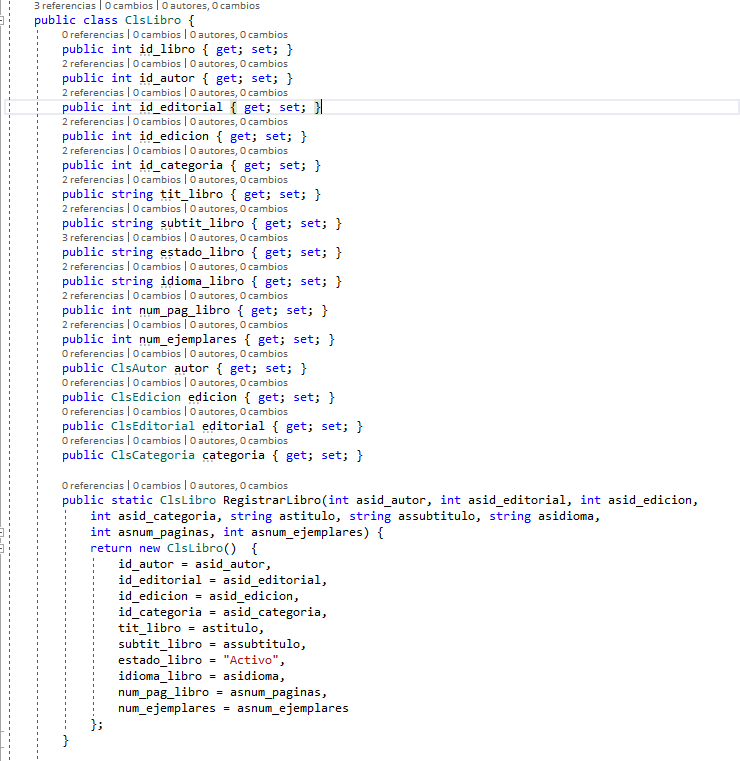
\includegraphics[width=4.91in,height=3.15in]{./media/8a.png}
	\end{Center}
	\begin{Center}
		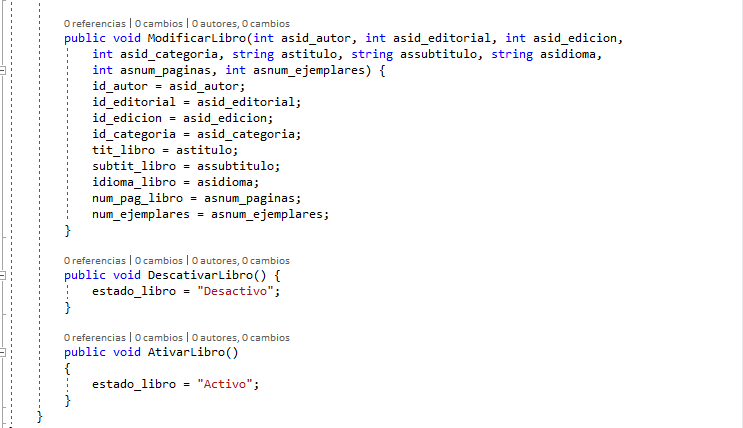
\includegraphics[width=4.91in,height=3.15in]{./media/8b.png}
	\end{Center}
\end{figure}

\newpage
Clase Persona:
\begin{figure}[H]
	\begin{Center}
		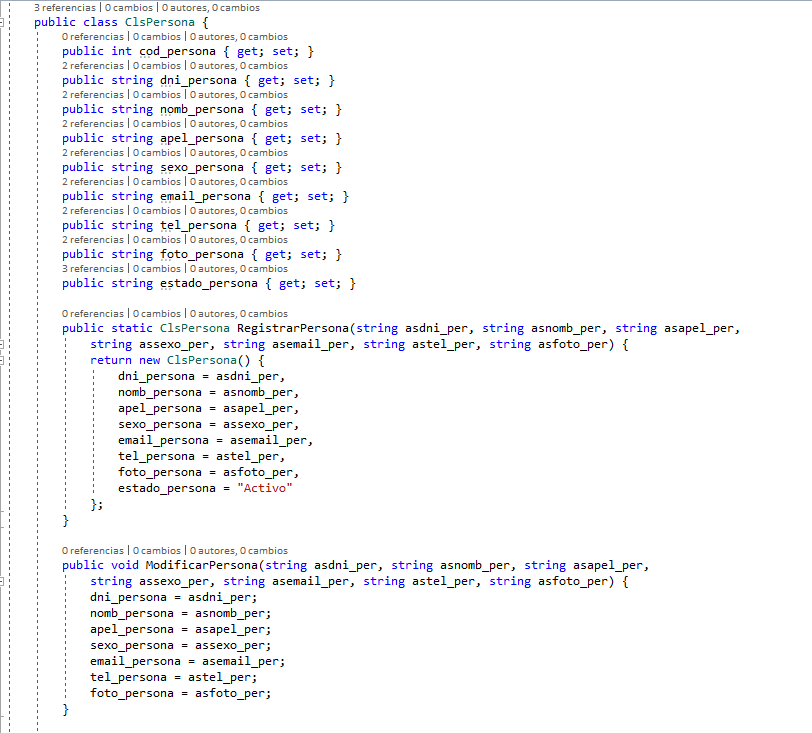
\includegraphics[width=4.91in,height=3.15in]{./media/9a.png}
	\end{Center}
	\begin{Center}
		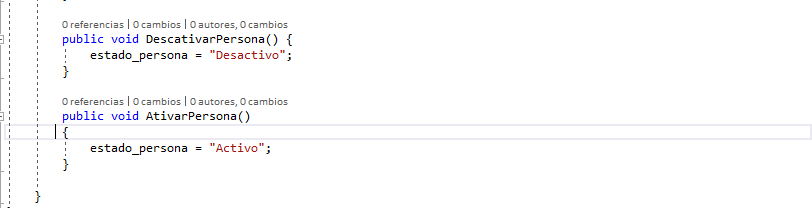
\includegraphics[width=4.91in,height=3.15in]{./media/9b.png}
	\end{Center}
\end{figure}

\newpage
Clase Prestamo:
\begin{figure}[H]
	\begin{Center}
		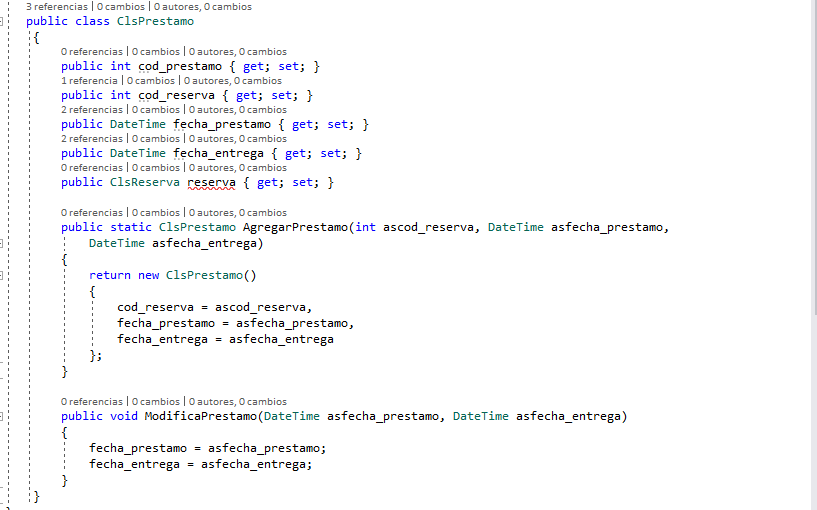
\includegraphics[width=4.91in,height=4.15in]{./media/10.png}
	\end{Center}
\end{figure}

Clase Rankingl:
\begin{figure}[H]
	\begin{Center}
		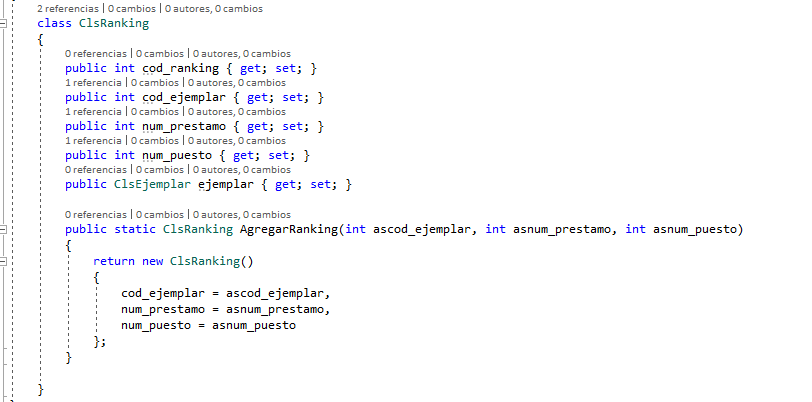
\includegraphics[width=4.91in,height=4.15in]{./media/11.png}
	\end{Center}
\end{figure}

\newpage
Clase Reserva:
\begin{figure}[H]
	\begin{Center}
		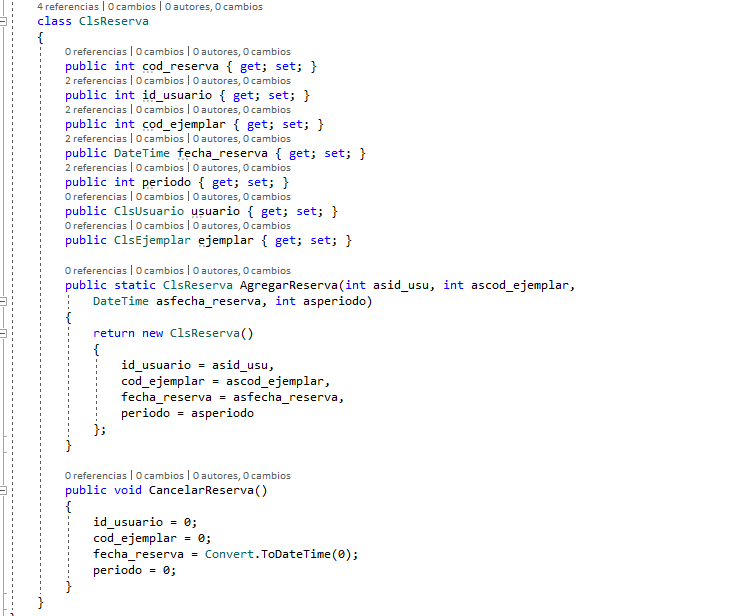
\includegraphics[width=4.91in,height=4.35in]{./media/12.png}
	\end{Center}
\end{figure}


Clase Tipo de Usuario:
\begin{figure}[H]
	\begin{Center}
		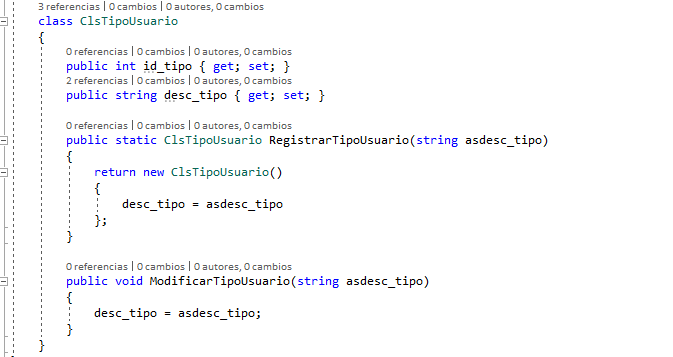
\includegraphics[width=4.91in,height=4.15in]{./media/13.png}
	\end{Center}
\end{figure}

\newpage
Clase Usuariol:
\begin{figure}[H]
	\begin{Center}
		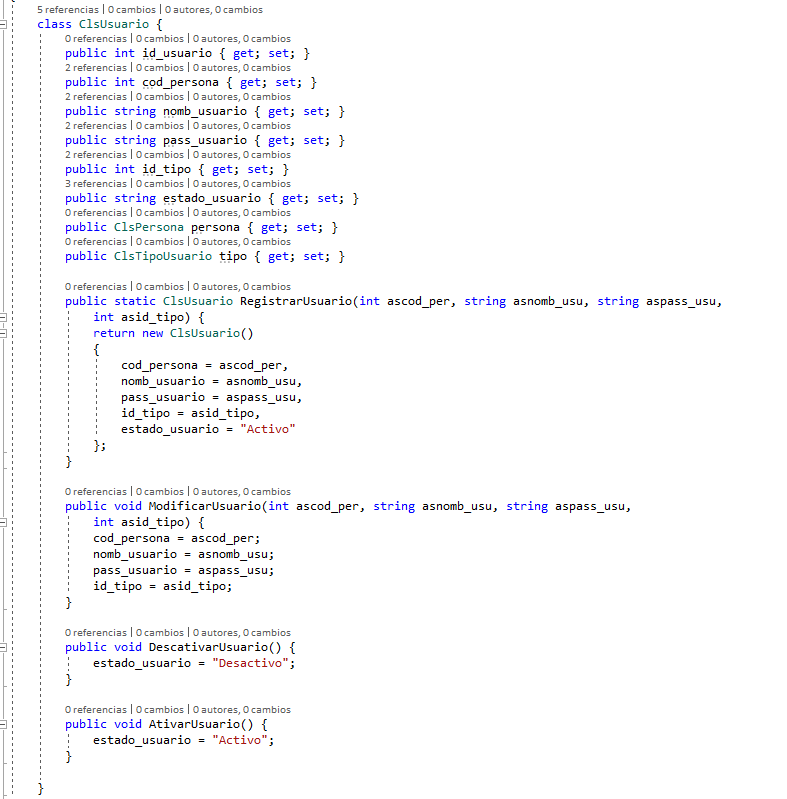
\includegraphics[width=4.91in,height=4.35in]{./media/14.png}
	\end{Center}
\end{figure}


\end{enumerate}
\end{enumerate}\par


\vspace{\baselineskip}

\vspace{\baselineskip}

\vspace{\baselineskip}

\vspace{\baselineskip}

\printbibliography
\end{document}